\documentclass[journal]{IEEEtran}
\usepackage{cite}
\usepackage{amsmath,amssymb,amsfonts}
\usepackage{algorithm}
\usepackage{algpseudocode}
\usepackage{graphicx}
\usepackage{xcolor}
\usepackage{booktabs}
\usepackage{tikz}
\usetikzlibrary{arrows.meta,backgrounds,fit}
\usepackage{pgfplots}
\pgfplotsset{compat=1.18}
\usepgfplotslibrary{groupplots}
\usepackage{url}
\usepackage[hidelinks]{hyperref}

\newtheorem{proposition}{Proposition}
\input{generated/results_macros}

\definecolor{cBlue}{RGB}{52,101,164}
\definecolor{cRed}{RGB}{196,78,82}
\definecolor{cGreen}{RGB}{85,153,96}
\definecolor{cOrange}{RGB}{221,132,52}
\definecolor{cPurple}{RGB}{129,114,179}
\definecolor{cGray}{RGB}{120,120,120}
\tikzset{box/.style={draw=#1!70!black,fill=#1!12,rounded corners=3pt,align=center,font=\footnotesize,minimum height=1.05cm,text width=2.85cm,line width=0.6pt},box/.default=cBlue,arr/.style={-{Stealth[length=2.2mm]},line width=0.6pt,draw=black!75},darr/.style={arr,dashed}}
\pgfplotsset{every axis/.append style={font=\footnotesize,grid=major,grid style={gray!25},legend style={font=\scriptsize,draw=gray!50,fill=white,fill opacity=0.9,text opacity=1}}}
\algrenewcommand\algorithmicrequire{\textbf{Input:}}
\algrenewcommand\algorithmicensure{\textbf{Output:}}

\begin{document}

\title{Sequence-Aware Learning for Energy-Efficient Software-Defined Networks: An Exact Oracle and an Empirical Study of When History Matters}

\author{Anonymous Authors%
\thanks{Author names and affiliations are withheld for review.}}

\markboth{IEEE Transactions on Green Communications and Networking}{Sequence-Aware Learning for Energy-Efficient SDNs}

\maketitle
\IEEEpeerreviewmaketitle

\begin{abstract}
Learned controllers for energy-aware software-defined networks (SDNs) usually map each traffic matrix to a precomputed link-sleeping configuration. Such snapshot decisions ignore the cost of changing configuration, which includes link wake-ups, flow-rule updates, and device wear. We formulate configuration as a sequential problem over a finite library of configurations. Energy, reconfiguration cost, and wear then form one objective that dynamic programming solves exactly, and we use this solution to train LiRA, a history-conditioned policy learned by imitation with dataset aggregation and a utilization safety layer. We then ask when sequence awareness pays off. On two real traces, Abilene and G\'{E}ANT, the optimal sequence is a single configuration: snapshot classifiers change configuration at most \abiBFourchg\ times per day, and LiRA reaches the oracle cost and is within 0.02\% of the snapshot classifiers, with energy savings of \abiSav\% and \geaSav\%. On a semi-synthetic Nobel-Germany trace with noisy demands, a gradient-boosted snapshot classifier changes configuration \nobBFourchg\ times per day (a random forest only \modRfChg\ times), and nearly every change saves less than one percent of the interval energy. LiRA reduces configuration changes and link transitions by \nobY\% at unchanged savings, yet a hysteresis rule tuned on validation data does as well (adjusted $p=\nobPbsix$). Under higher load, LiRA reaches the oracle cost (\nobhlJLiRA\ against \nobhlJBSix\ for hysteresis), but the difference is not significant over \nobTestDays\ test days. The oracle agrees with an independent mixed-integer program to $\dpMilpDiff$, and a Mininet emulation of \emuTrans\ transitions shows that each change takes about \emuTransS\\,s and loses a few probe packets. Our results show that sequence awareness matters for classifiers that flap and for noisy demands, and that on smooth real traffic a simple snapshot rule already suffices.
\end{abstract}

\begin{IEEEkeywords}
Software-defined networking, energy efficiency, link sleeping, imitation learning, dynamic programming, reconfiguration cost, device lifetime, negative results.
\end{IEEEkeywords}

\section{Introduction}

\IEEEPARstart{B}{ackbone} and data-center links are provisioned for peak demand, yet their average utilization is far lower, so a large share of the power drawn by line cards and transceivers is spent carrying little or no traffic. Putting idle links to sleep was proposed more than two decades ago~\cite{gupta2003greening} and has since grown into a broad research area~\cite{bianzino2012survey,bolla2011energy}. Software-defined networking (SDN) makes the idea practical, because a logically centralized controller can observe the traffic matrix and switch link power states and forwarding rules network-wide~\cite{mckeown2008openflow,kreutz2015sdn}. The underlying optimization is a mixed-integer problem that is NP-hard in general~\cite{chiaraviglio2012minimizing}, and exact solvers need seconds per traffic matrix on realistic topologies (Section~\ref{sec:res-time}), which is slow for control loops that run every few minutes.

Recent work closes this speed gap with machine learning. A model is trained offline to map each incoming traffic matrix to one of a set of precomputed, energy-efficient configurations, which replaces the integer program at run time~\cite{gomezdelahiz2025noms,gomezdelahiz2026tgcn}. The same pattern of replacing a solver with a learned mapping appears in traffic engineering~\cite{xu2023teal,perry2023dote,abuzaid2021ncflow,almasan2022enero} and in combinatorial optimization more broadly~\cite{bengio2021mlco}.

A snapshot decision treats every interval as the first. The configuration chosen for the current traffic matrix ignores which configuration is installed, although moving between configurations has costs. Links must be woken or put to sleep, flow tables must be rewritten, and updates that are not carefully ordered can cause transient loops or loss~\cite{reitblatt2012abstractions,jin2014dionysus}. Each power-state transition also adds a thermal cycle that can offset the lifetime benefit of sleeping~\cite{chiaraviglio2015lifetime,chiaraviglio2014impact}. The natural hypothesis is that snapshot classifiers flap between neighboring configurations when demand hovers near a decision boundary, and that a sequence-aware method should avoid this at little cost in energy.

This paper tests that hypothesis rather than assuming it. We make four contributions.

\begin{itemize}
\item \emph{Formulation and exact oracle.} We formulate energy-aware configuration as a sequential problem that jointly prices energy, reconfiguration, and wear. Over a finite library, the problem is a shortest path on a trellis, which dynamic programming solves exactly in $O(TK^2)$ time. We validate the solver against an independent mixed-integer program to $\dpMilpDiff$ and prove that snapshot decisions can have regret that grows linearly with the horizon (Sections~\ref{sec:problem} and~\ref{sec:framework}).
\item \emph{A sequence-aware learner.} LiRA imitates the oracle with cost-sensitive weights and dataset aggregation (DAgger)~\cite{ross2011dagger}, conditions on the installed configuration and its dwell time, and wraps the policy in a feasibility safety layer. Drift detectors that trigger retraining are included as a component, and Section~\ref{sec:res-main} reports that our drift study does not validate them (Sections~\ref{sec:framework} and~\ref{sec:algorithms}).
\item \emph{A broad empirical study with negative and positive findings.} We evaluate on Abilene, G\'{E}ANT, and a semi-synthetic Nobel-Germany series under four load and power scenarios, against snapshot learning, hysteresis, minimum-dwell, rolling-horizon, integer-programming, genetic-algorithm, and greedy baselines, with ablations, sensitivity analyses, a drift study, and rolling-origin folds (Sections~\ref{sec:setup} and~\ref{sec:results}).
\item \emph{Emulation of transition cost.} A Mininet and Open vSwitch emulation replays the most active day of the Nobel-Germany series and measures rule-installation time, transition duration, probe loss, and delay for each method (Section~\ref{sec:res-emu}).
\end{itemize}

Our findings are mixed, and we report them as measured. On the two real traces, the energy-optimal configuration changes rarely: the exact oracle uses one configuration for the whole test period, snapshot classifiers change configuration at most \abiBFourchg\ times per day, and LiRA, hysteresis, and the snapshot classifier reach the same energy savings (\abiSav\% on Abilene and \geaSav\% on G\'{E}ANT) and the same cost. LiRA therefore offers no measurable advantage there. On the Nobel-Germany series, whose demands are noisy, the snapshot classifier flaps (\nobBFourchg\ changes per day), nearly every change saves less than one percent of the interval energy, and LiRA removes \nobY\% of the changes. A hysteresis rule tuned on validation data achieves the same, and the only setting in which LiRA is better than tuned hysteresis in cost (higher load, \nobhlJLiRA\ against \nobhlJBSix) is not statistically significant. The practical conclusion is that the benefit of sequence awareness depends on the traffic and on the classifier. It is large for a flapping classifier, and it is negligible for smooth real traffic, where a snapshot rule and a hysteresis guard already suffice.

The remainder of the paper reviews related work (Section~\ref{sec:related}), formulates the problem (Section~\ref{sec:problem}), presents LiRA (Sections~\ref{sec:framework} and~\ref{sec:algorithms}), describes the setup (Section~\ref{sec:setup}), reports results (Section~\ref{sec:results}), and discusses implications, limitations, and conclusions (Sections~\ref{sec:discussion}--\ref{sec:conclusion}).

\section{Related Work}\label{sec:related}

\subsection{Energy-Aware Networking and Sleep Modes}

Surveys of green networking classify techniques into adaptive link rate, sleeping, and energy-aware routing~\cite{bianzino2012survey,bolla2011energy}. Chiaraviglio \emph{et al.} formulated ISP energy minimization as an integer program and proposed heuristics that switch off nodes and links subject to capacity and connectivity constraints~\cite{chiaraviglio2012minimizing}. GreenTE maximizes the number of links that can sleep under utilization and delay constraints~\cite{zhang2010greente}, ElasticTree applies the same principle to data-center networks~\cite{heller2010elastictree}, and EATe spreads traffic online so that lightly loaded links can sleep~\cite{vasic2010eate}. Power models for such studies rely on measured device profiles~\cite{mahadevan2009power,restrepo2009energy,vishwanath2014modeling}. In SDN, energy-aware routing has been formulated as integer programs with heuristics for carrier-grade Ethernet~\cite{maaloul2018carrier}, and a survey of SDN-specific methods is given in~\cite{assefa2019survey}.

\subsection{Learning for Energy-Efficient Networking}

MER-SDN uses machine learning to predict the parameters of an energy-aware routing heuristic~\cite{assefa2018mersdn}. Reinforcement learning has been applied in an SDN controller to trade packet delay against energy~\cite{frohlich2021rl} and to compute energy-saving routes in data-center networks~\cite{zheng2022energysaving}. In cellular networks, deep reinforcement learning combined with traffic forecasting controls base-station sleep modes~\cite{wu2021deepbsc}, a problem that shares the on-off structure of link sleeping. The closest works to ours replace the optimizer with a learned mapping from traffic matrices to precomputed configurations and report large speedups~\cite{gomezdelahiz2025noms,gomezdelahiz2026tgcn}. We reimplement this snapshot approach as baseline B4 with our own library, features, and classifier, because we could not run the original code. The comparison therefore concerns the snapshot principle and not the exact published systems.

\subsection{Learning to Optimize and Learned Traffic Engineering}

Machine learning for combinatorial optimization treats problem instances as data and learns to imitate expert decisions or to replace parts of a solver~\cite{bengio2021mlco}. In traffic engineering, learning-accelerated and decomposition-based solvers~\cite{xu2023teal,perry2023dote,abuzaid2021ncflow,narayanan2021pop}, learned routing~\cite{valadarsky2017learning}, deep reinforcement learning with graph neural networks~\cite{almasan2022enero,bernardez2023magnneto}, and neural models of network performance~\cite{rusek2020routenet} have shown that learned components can approach solver quality at much lower latency. These methods optimize each traffic matrix independently. LiRA instead imitates an oracle that is exact for the sequential objective, which the finite library makes tractable offline.

\subsection{Reconfiguration Cost, Device Lifetime, and Switching Costs}

Consistent-update abstractions~\cite{reitblatt2012abstractions} and update scheduling~\cite{jin2014dionysus} show that changing forwarding state is neither free nor instantaneous. Bonetto \emph{et al.} included reconfiguration costs in multi-period power-aware logical topology design~\cite{bonetto2013multiperiod}. Chiaraviglio \emph{et al.} modeled how sleep modes affect device lifetime through temperature and power-state transitions~\cite{chiaraviglio2015lifetime,chiaraviglio2014impact}, and lifetime-aware provisioning has been studied for optical backbones~\cite{wiatr2016lifetime}. Online problems with switching costs are studied as metrical task systems~\cite{borodin1992mts} and smoothed online convex optimization~\cite{chen2018obd}, with dynamic right-sizing of data centers as a well-known application~\cite{lin2013rightsizing}. Our setting is a metrical task system with a finite state space whose offline optimum is computable, which makes imitation learning natural~\cite{ross2011dagger}. Concept-drift adaptation~\cite{gama2014drift,lu2019drift} with detectors such as ADWIN~\cite{bifet2007adwin} and cumulative-sum tests~\cite{page1954cusum} provides the tools for deciding when to retrain, and drift is known to degrade learned models in network security~\cite{andresini2021insomnia}.

\section{Problem Formulation}\label{sec:problem}

Table~\ref{tab:notation} summarizes the notation.

\begin{table}[t]
\centering
\caption{Main Notation}
\label{tab:notation}
\footnotesize
\setlength{\tabcolsep}{3pt}
\begin{tabular}{@{}p{1.85cm}p{6.5cm}@{}}
\toprule
Symbol & Meaning \\
\midrule
$G=(V,E)$ & Network graph; $E$ is the set of undirected links \\
$\kappa_e$ & Capacity of link $e$ in each direction \\
$\Delta$, $n_d$ & Control interval; number of intervals per day \\
$D_t$ & Traffic matrix of interval $t$ \\
$c=(x,r)$ & Configuration: link states $x\in\{0,1\}^{|E|}$, routing $r$ \\
$\mathcal{C}$, $K$ & Configuration library and its size \\
$u_e$, $\theta$ & Utilization of link $e$; utilization threshold \\
$E(c,D)$ & Energy of $c$ under traffic $D$ in one interval \\
$R(c',c)$ & Reconfiguration cost of moving from $c'$ to $c$ \\
$\mathrm{AF}_e$, $\alpha$, $\chi$ & Acceleration factor; sleep factor; cycling weight \\
$W(c',c)$ & Per-step wear cost \\
$\lambda_R,\lambda_W$ & Prices of reconfiguration and wear \\
$J$, $V_t$, $Q_t$ & Total cost; cost-to-go; action value \\
\bottomrule
\end{tabular}
\end{table}

\subsection{Configuration Model}

The network is a graph $G=(V,E)$ in which each undirected link $e$ has capacity $\kappa_e$ in each direction and consists of two ports that sleep and wake together. Time is divided into control intervals of length $\Delta$, and $D_t$ is the traffic matrix of interval $t$. A configuration $c=(x,r)$ consists of a link-state vector $x\in\{0,1\}^{|E|}$, with $x_e=1$ for an active link, and a routing $r$ that splits each origin--destination demand over up to $k$ precomputed paths that use only active links. A library $\mathcal{C}=\{c_1,\dots,c_K\}$ of such configurations is built offline (Section~\ref{sec:library}). The utilization $u_e(c,D)$ of link $e$ in a direction is the offered load divided by $\kappa_e$, and $c$ is feasible for $D$ if
\begin{equation}\label{eq:mlu}
\mathrm{MLU}(c,D)=\max_{e:\,x_e=1,\ \mathrm{dir}}u_e(c,D)\le\theta
\end{equation}
for a utilization threshold $\theta<1$.

\subsection{Energy Model}

Chassis stay powered, so the controllable power is that of link ports. Following load-dependent port profiles~\cite{restrepo2009energy,mahadevan2009power,vishwanath2014modeling}, the energy of $c$ in interval $t$ is
\begin{equation}\label{eq:energy}
\begin{split}E(c,D_t)=\Delta\sum_{e\in E}\Big[&x_e\big(2P^{\mathrm{idle}}+P^{\mathrm{dyn}}(u_e^{\rightarrow}+u_e^{\leftarrow})\big)\\
&+(1-x_e)\,2P^{\mathrm{sl}}\Big],\end{split}
\end{equation}
where $P^{\mathrm{idle}}$, $P^{\mathrm{dyn}}$, and $P^{\mathrm{sl}}$ are the idle, full-load dynamic, and sleep power of one port, and $u_e^{\rightarrow},u_e^{\leftarrow}$ are the directional utilizations. We report energy in units of one interval of the idle power of all links, so that the energy of the all-on configuration is close to one per interval.

\subsection{Reconfiguration Cost}

Moving from $c'$ to $c$ toggles $\|x-x'\|_1$ links, changes $\Delta F(c',c)$ forwarding entries (the number of switch and origin--destination pairs whose next hops differ), and moves a share $B(c',c)\in[0,1]$ of the traffic to different paths. The reconfiguration cost is
\begin{equation}\label{eq:reconf}
R(c',c)=\tfrac13\Big[\frac{\|x-x'\|_1}{\rho_1}+\frac{\Delta F(c',c)}{\rho_2}+\frac{B(c',c)}{\rho_3}\Big],
\end{equation}
where $\rho_1,\rho_2,\rho_3$ are the 95th percentiles of the three terms over distinct library pairs, so that a typical large change costs about one unit.

\subsection{Wear Model}

We adopt the acceleration-factor view of Chiaraviglio \emph{et al.}~\cite{chiaraviglio2015lifetime}: relative to an always-on device, sleeping lowers the failure rate, whereas power-state transitions raise it through thermal cycling. Let $\tau_e$ be the fraction of time link $e$ sleeps and $f_e$ its number of transitions per day. We use the linear form
\begin{equation}\label{eq:af}
\mathrm{AF}_e=(1-\tau_e)+\alpha\,\tau_e+\chi f_e=1-(1-\alpha)\tau_e+\chi f_e,
\end{equation}
where $\alpha<1$ is the relative failure rate while asleep and $\chi$ weighs one transition per day. A value $\mathrm{AF}_e>1$ means that the link ages faster than an always-on link. Over a horizon of $T$ intervals, $\sum_{t}W(c_{t-1},c_t)=\frac{T}{n_d}\sum_e(\mathrm{AF}_e-1)$ for the additive per-step term
\begin{equation}\label{eq:wear}
W(c',c)=\sum_{e\in E}\Big[\chi\,|x_e-x'_e|-\frac{1-\alpha}{n_d}(1-x_e)\Big].
\end{equation}
This decomposition is exact and makes wear additive over time. The parameters $\alpha$ and $\chi$ are assumed, representative values (Section~\ref{sec:params}), and we study the sensitivity of the results to them.

\subsection{Sequential Objective}

Given an initial configuration $c_0$, the sequential problem selects $c_1,\dots,c_T\in\mathcal{C}$ that minimize
\begin{equation}\label{eq:objective}
J(c_{1:T})=\sum_{t=1}^{T}\Big[E(c_t,D_t)+\lambda_R R(c_{t-1},c_t)+\lambda_W W(c_{t-1},c_t)\Big]
\end{equation}
subject to \eqref{eq:mlu} in every interval, where $\lambda_R,\lambda_W\ge0$ set the price of reconfiguration and wear relative to energy. Snapshot methods instead use the per-interval rule
\begin{equation}\label{eq:snapshot}
c^{\mathrm{snap}}_t=\arg\min_{c\in\mathcal{C}:\,\mathrm{MLU}(c,D_t)\le\theta}E(c,D_t),
\end{equation}
which ignores the installed configuration. Online, the controller uses an estimate of $D_t$ from flow counters or link loads~\cite{zhang2003tomogravity}.

\subsection{Cost of Ignoring the Sequence}

For two configurations $c_a$ and $c_b$, let $s_{ab}=\lambda_R R(c_a,c_b)+\lambda_W\chi\|x_a-x_b\|_1$ be the non-energy cost of switching between them.

\begin{proposition}\label{prop:snapshot}
Let $c_a,c_b\in\mathcal{C}$ be feasible in every interval and have the same number of sleeping links, and let the traffic alternate so that $E(c_a,D_t)-E(c_b,D_t)=(-1)^t\epsilon$ with $\epsilon>0$, while every other library member is dominated in every interval. Then the snapshot rule \eqref{eq:snapshot} incurs a regret of at least $(T-1)s_{ab}-\lceil T/2\rceil\epsilon$ with respect to the optimum of \eqref{eq:objective}, which grows linearly in $T$ whenever $s_{ab}>\epsilon/2$.
\end{proposition}
\begin{IEEEproof}
The snapshot rule selects $c_b$ in even and $c_a$ in odd intervals, so it pays the lower energy in each interval and switches $T-1$ times. The sleep terms of \eqref{eq:wear} are identical for $c_a$ and $c_b$, so the two sequences differ only in energy and in switching cost. Staying at $c_a$ throughout pays at most $\lceil T/2\rceil\epsilon$ more energy and never switches. Its cost is an upper bound on the optimum, which proves the claim.
\end{IEEEproof}

The proposition shows that flapping can be costly in principle. Whether it is costly in practice depends on whether real traffic produces such near-ties, which is the empirical question of Section~\ref{sec:results}.

\section{LiRA: Framework and Analysis}\label{sec:framework}

Fig.~\ref{fig:arch} shows the architecture. An offline plane builds the configuration library, computes sequence-optimal labels with the dynamic-programming oracle, and trains the policy. An online plane runs once per interval: it estimates the traffic matrix, builds features, queries the policy, checks feasibility, and installs only the difference between the current and the new configuration. Drift detectors connect the two planes.

\begin{figure*}[t]
\centering
\resizebox{\textwidth}{!}{%
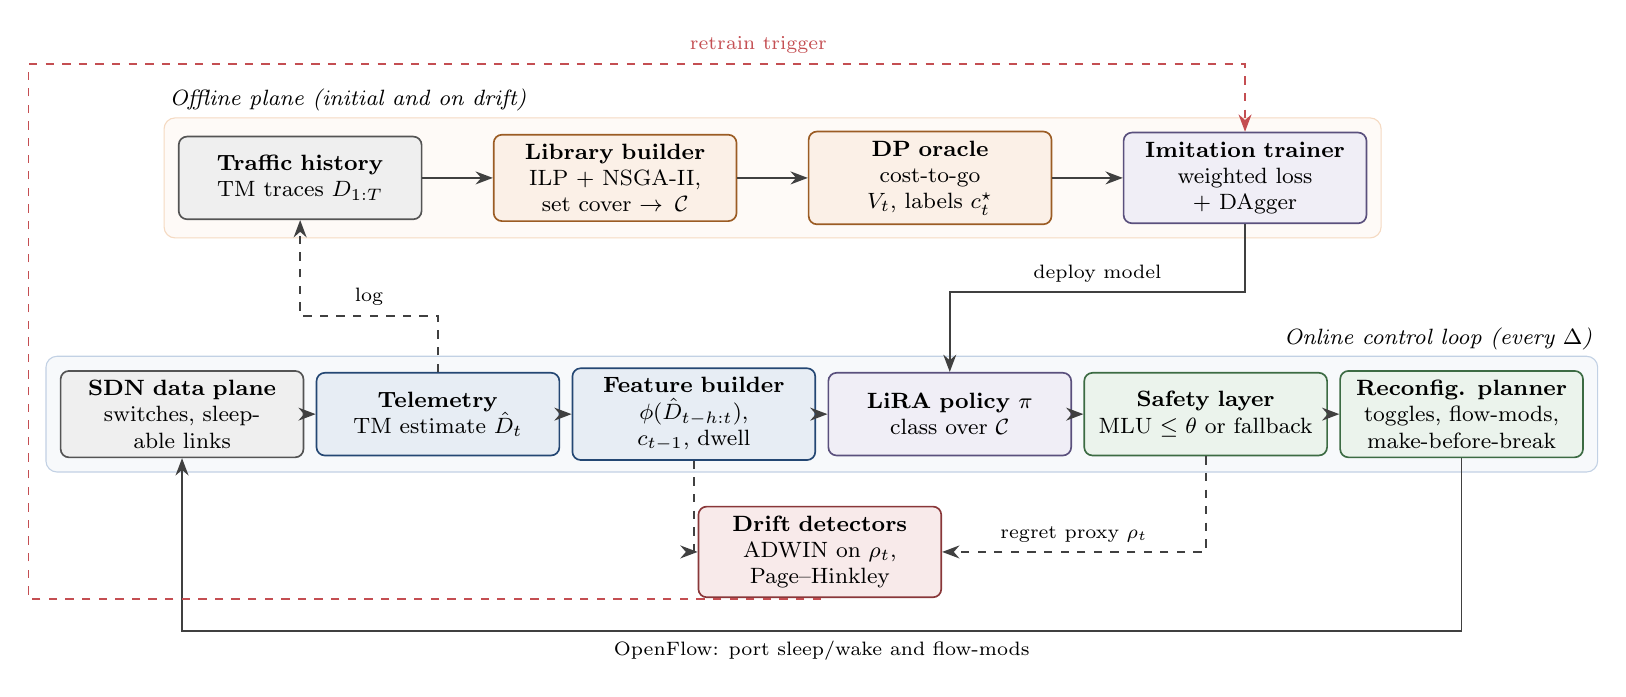
\begin{tikzpicture}
\node[box=cGray] (hist) at (1.5,3.0) {\textbf{Traffic history}\\TM traces $D_{1:T}$};
\node[box=cOrange] (lib) at (5.5,3.0) {\textbf{Library builder}\\ILP + NSGA-II, set cover $\rightarrow\mathcal{C}$};
\node[box=cOrange] (dp) at (9.5,3.0) {\textbf{DP oracle}\\cost-to-go $V_t$, labels $c^\star_t$};
\node[box=cPurple] (train) at (13.5,3.0) {\textbf{Imitation trainer}\\weighted loss + DAgger};
\node[box=cGray] (dpl) at (0,0) {\textbf{SDN data plane}\\switches, sleepable links};
\node[box] (tel) at (3.25,0) {\textbf{Telemetry}\\TM estimate $\hat{D}_t$};
\node[box] (feat) at (6.5,0) {\textbf{Feature builder}\\$\phi(\hat{D}_{t-h:t})$, $c_{t-1}$, dwell};
\node[box=cPurple] (pol) at (9.75,0) {\textbf{LiRA policy} $\pi$\\class over $\mathcal{C}$};
\node[box=cGreen] (safe) at (13,0) {\textbf{Safety layer}\\$\mathrm{MLU}\le\theta$ or fallback};
\node[box=cGreen] (plan) at (16.25,0) {\textbf{Reconfig. planner}\\toggles, flow-mods, make-before-break};
\node[box=cRed] (drift) at (8.1,-1.75) {\textbf{Drift detectors}\\ADWIN on $\rho_t$, Page--Hinkley};
\begin{scope}[on background layer]
\node[fill=cOrange!4,draw=cOrange!30,rounded corners=4pt,inner sep=5pt,fit=(hist)(train),label={[font=\footnotesize\itshape,anchor=south west,inner sep=2pt]north west:Offline plane (initial and on drift)}] {};
\node[fill=cBlue!4,draw=cBlue!30,rounded corners=4pt,inner sep=5pt,fit=(dpl)(plan),label={[font=\footnotesize\itshape,anchor=south east,inner sep=2pt]north east:Online control loop (every $\Delta$)}] {};
\end{scope}
\draw[arr] (hist) -- (lib);
\draw[arr] (lib) -- (dp);
\draw[arr] (dp) -- (train);
\draw[arr] (dpl) -- (tel);
\draw[arr] (tel) -- (feat);
\draw[arr] (feat) -- (pol);
\draw[arr] (pol) -- (safe);
\draw[arr] (safe) -- (plan);
\draw[arr] (train.south) -- (13.5,1.55) -- node[above,font=\scriptsize,pos=0.5]{deploy model} (9.75,1.55) -- (pol.north);
\draw[darr] (tel.north) -- (3.25,1.25) -- node[above,font=\scriptsize]{log} (1.5,1.25) -- (hist.south);
\draw[arr] (plan.south) -- (16.25,-2.75) -- node[below,font=\scriptsize]{OpenFlow: port sleep/wake and flow-mods} (0,-2.75) -- (dpl.south);
\draw[darr] (feat.south) -- (6.5,-1.75) -- (drift.west);
\draw[darr] (safe.south) -- (13,-1.75) -- node[above,font=\scriptsize]{regret proxy $\rho_t$} (drift.east);
\draw[darr,draw=cRed] (drift.south) -- (8.1,-2.35) -- (-1.95,-2.35) -- (-1.95,4.45) -- node[above,font=\scriptsize,text=cRed,pos=0.6]{retrain trigger} (13.5,4.45) -- (train.north);
\end{tikzpicture}}
\caption{Architecture of LiRA. The offline plane builds the configuration library, computes sequence-optimal labels with the dynamic-programming oracle, and trains the policy. The online loop estimates the traffic matrix, selects a configuration conditioned on the installed one, enforces the utilization bound, and installs only the configuration difference. Drift detectors trigger retraining.}
\label{fig:arch}
\end{figure*}

\subsection{Configuration Library}\label{sec:library}

The library must be small enough for fast decisions and rich enough to contain an efficient feasible configuration for almost every traffic matrix. We cluster training traffic matrices with $k$-means ($64$ clusters) and take the element-wise 95th-percentile matrix of each cluster as its representative. For each representative we solve the path-based energy-minimization integer program with $k=4$ shortest paths, link-pair sleeping, connectivity, and the bound \eqref{eq:mlu}, and we run NSGA-II~\cite{deb2002nsga2} on port count and maximum utilization to add Pareto-diverse link-state vectors. For Abilene, whose link-state space is small, we also enumerate all connected link states. Duplicate vectors are merged, the routing of each vector is re-optimized by a linear program that minimizes maximum utilization, and further integer programs are solved for uncovered training and validation matrices until at least 99.5\% are covered. The all-on configuration is always included. The library is pruned to $K$ configurations by greedy energy coverage on every sixth training interval.

\subsection{Exact Sequence-Optimal Oracle}

Because all terms of \eqref{eq:objective} depend only on $(c_{t-1},c_t,D_t)$, the problem is a shortest path through a trellis whose stages are intervals and whose states are library members (Fig.~\ref{fig:trellis}). Infeasible states receive infinite cost. The backward recursion
\begin{equation}\label{eq:dp}
\begin{aligned}V_{t-1}(c')&=\min_{c\in\mathcal{C}}Q_t(c',c),\\
Q_t(c',c)&=E(c,D_t)+\lambda_R R(c',c)+\lambda_W W(c',c)+V_t(c)\end{aligned}
\end{equation}
computes the cost-to-go $V_t(c)$ of being in $c$ at the end of interval $t$, with $V_T\equiv0$. The oracle trajectory follows $c^\star_t=\arg\min_c Q_t(c^\star_{t-1},c)$. The table $Q_t(c',\cdot)$ also gives the optimal action for \emph{any} installed configuration $c'$, which we use to relabel states visited by the learner.

\begin{proposition}\label{prop:dp}
For a fixed library $\mathcal{C}$ and known $D_{1:T}$, recursion \eqref{eq:dp} returns a feasible sequence minimizing \eqref{eq:objective} whenever one exists, in $O(TK^2)$ time and $O(TK)$ memory.
\end{proposition}
\begin{IEEEproof}
By \eqref{eq:wear}, the wear contribution is a sum of terms that each depend on one pair of consecutive configurations, and \eqref{eq:energy} and \eqref{eq:reconf} depend on $(c_{t-1},c_t,D_t)$ only. Hence \eqref{eq:objective} is the length of a path through a layered graph with $K$ nodes per layer, and edges into infeasible nodes have infinite weight. Bellman's principle of optimality yields \eqref{eq:dp}, and each layer requires $K^2$ evaluations of precomputed quantities.
\end{IEEEproof}

\begin{figure}[t]
\centering
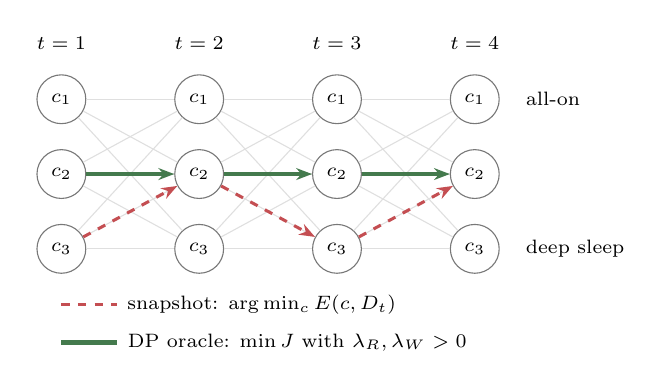
\begin{tikzpicture}[st/.style={circle,draw=cGray,fill=white,minimum size=0.62cm,inner sep=0pt,font=\scriptsize},x=1.75cm,y=0.95cm]
\foreach \t in {1,...,4}{\node[font=\scriptsize] at (\t,0.75) {$t=\t$};}
\foreach \t in {1,...,4}{\foreach \c/\y in {1/0,2/-1,3/-2}{\node[st] (n\t\c) at (\t,\y) {$c_{\c}$};}}
\foreach \t/\u in {1/2,2/3,3/4}{\foreach \a in {1,2,3}{\foreach \b in {1,2,3}{\draw[gray!25,line width=0.4pt] (n\t\a) -- (n\u\b);}}}
\draw[cRed,line width=1.1pt,dashed,-{Stealth[length=2mm]}] (n13) -- (n22);
\draw[cRed,line width=1.1pt,dashed,-{Stealth[length=2mm]}] (n22) -- (n33);
\draw[cRed,line width=1.1pt,dashed,-{Stealth[length=2mm]}] (n33) -- (n42);
\draw[cGreen!80!black,line width=1.6pt,-{Stealth[length=2mm]}] (n12) -- (n22);
\draw[cGreen!80!black,line width=1.6pt,-{Stealth[length=2mm]}] (n22) -- (n32);
\draw[cGreen!80!black,line width=1.6pt,-{Stealth[length=2mm]}] (n32) -- (n42);
\node[font=\scriptsize,anchor=west] at (4.3,0) {all-on};
\node[font=\scriptsize,anchor=west] at (4.3,-2) {deep sleep};
\draw[cRed,line width=1.1pt,dashed] (1.0,-2.75) -- (1.4,-2.75) node[right,font=\scriptsize,text=black] {snapshot: $\arg\min_c E(c,D_t)$};
\draw[cGreen!80!black,line width=1.6pt] (1.0,-3.25) -- (1.4,-3.25) node[right,font=\scriptsize,text=black] {DP oracle: $\min J$ with $\lambda_R,\lambda_W>0$};
\end{tikzpicture}
\caption{Configuration trellis (schematic). Nodes are library configurations per interval, and edges carry reconfiguration and wear costs. Snapshot selection flaps between $c_2$ and $c_3$ when traffic hovers near a decision boundary, whereas the oracle keeps $c_2$ when the extra energy is smaller than the switching cost.}
\label{fig:trellis}
\end{figure}

\subsection{History-Conditioned Policy}

The policy maps the input $s_t$ to a library index. The input contains the principal components (95\% variance, fitted on training data) of the log-scaled origin--destination vector, the total volume, the shares of the ten largest demands, time of day and day of week, the changes of the principal components and the volume over the last $1$, $3$, and $6$ intervals, the one-hot encoding of the installed configuration $c_{t-1}$, and its dwell time $\delta_{t-1}$ in intervals. The default model is a gradient-boosted tree classifier (XGBoost~\cite{chen2016xgboost}), and Section~\ref{sec:res-models} compares LightGBM~\cite{ke2017lightgbm}, random forests~\cite{breiman2001rf}, and a multilayer perceptron.

\textbf{Cost-sensitive imitation.} Plain classification treats all mistakes as equal, although choosing an action that is almost as cheap as the optimum is harmless. For each training state $(t,c')$ we compute the oracle action $a^\star=\arg\min_c Q_t(c',c)$ and the cost gap $g_t(c')=\min_{c\neq a^\star}Q_t(c',c)-Q_t(c',a^\star)$ to the second-best action. The classifier is trained with the sample weight $w=\mathrm{clip}(g/\bar g,0.2,5)$, where $\bar g$ is the mean gap, so that decisions with a large cost difference matter more. This weighted cross-entropy loss is a practical surrogate for a cost-sensitive classifier.

\textbf{DAgger.} A policy trained only on oracle trajectories never sees the states that its own mistakes create. We apply DAgger~\cite{ross2011dagger} with three rounds: the current policy is rolled out on the training period, with the expert action used with probability $\beta_n=0.5\cdot0.5^{\,n-1}$ in round $n$, the visited pairs $(t,c_{t-1})$ are relabeled from the stored $Q$ tables without solving any new problem, and the policy is retrained on the aggregated data. Among the rounds, we keep the policy with the lowest sequence cost on the validation period.

\textbf{Guarantee.} Because the oracle is optimal from every state, the analysis of DAgger applies. Let $u=\max_{t,c',c}[Q_t(c',c)-\min_{\tilde c}Q_t(c',\tilde c)]$ bound the cost of one deviation from the oracle.

\begin{proposition}\label{prop:imitation}
Let $\epsilon_N$ be the smallest expected disagreement with the oracle, over the policy class, on the aggregated state distribution after $N$ DAgger rounds, measured with a cost-sensitive loss. For $N$ large enough, the analysis of~\cite{ross2011dagger} guarantees a policy $\hat\pi$ among the iterates with $J(\hat\pi)\le J^\star+uT\epsilon_N+O(1)$, where $J^\star$ is the oracle cost.
\end{proposition}
\begin{IEEEproof}
This is the DAgger guarantee for task costs, which holds because a single deviation from the expert increases the expert's cost-to-go by at most $u$.
\end{IEEEproof}

The bound is linear in the disagreement $\epsilon_N$ rather than quadratic in $T$, as it would be for behavior cloning alone. Our weighted cross-entropy loss only approximates the cost-sensitive loss assumed by the analysis, so the proposition is a motivation and not a guarantee for the implemented learner.

\subsection{Safety Layer}

At run time, the configuration chosen by the policy is checked against \eqref{eq:mlu} using the traffic estimate. If it is infeasible, the controller falls back to
\begin{equation}\label{eq:fallback}
\begin{split}c_t=\mathop{\arg\min}_{c\in\mathcal{C}:\,\mathrm{MLU}(c,\hat D_t)\le\theta}\Big[&E(c,\hat D_t)+\lambda_R R(c_{t-1},c)\\
&+\lambda_W W(c_{t-1},c)\Big],\end{split}
\end{equation}
which is evaluated for all $K$ configurations. If no configuration is feasible, the all-on configuration is used and the interval is counted as a violation.
\begin{proposition}\label{prop:safety}
If the all-on configuration satisfies $\mathrm{MLU}\le\theta$ for $\hat D_t$, the safety layer returns a configuration that satisfies \eqref{eq:mlu} for $\hat D_t$.
\end{proposition}
\begin{IEEEproof}
The all-on configuration belongs to $\mathcal{C}$ by construction, so the feasible set in \eqref{eq:fallback} is non-empty whenever the policy's choice is infeasible.
\end{IEEEproof}
The guarantee holds for the estimate $\hat D_t$. In our evaluation the estimate equals the realized matrix, so violations occur only when no library member is feasible.

\subsection{Drift Detection and Retraining}\label{sec:drift}

The oracle cannot be computed online, but a myopic regret proxy can. After each decision, the controller computes
\begin{equation}\label{eq:proxy}
\begin{split}\rho_t=&E(c_t,D_t)-\min_{c\in\mathcal{C}:\,\mathrm{MLU}(c,D_t)\le\theta}E(c,D_t)\\
&+\mathbb{1}[\mathrm{MLU}(c_t,D_t)>\theta],\end{split}
\end{equation}
the energy lost against the best feasible configuration plus a violation indicator. ADWIN~\cite{bifet2007adwin} monitors $\rho_t$, and a Page--Hinkley test~\cite{page1954cusum} monitors the deseasonalized log of the total traffic volume, that is, the log volume minus its training mean for the same time of week. When a detector fires, the policy is retrained on the last seven days with oracle labels computed on that window. Because the window just after a change still contains mostly old data, retraining is repeated one and three days later. A library refresh, which adds integer-program solutions for eight clusters of the recent window, is available as an option.

\section{Algorithms}\label{sec:algorithms}

Algorithm~\ref{alg:offline} summarizes offline training and Algorithm~\ref{alg:online} the online loop. Reconfigurations follow a make-before-break order: links that the new configuration needs are woken first, new rules are installed, and only then are unused links put to sleep.

\begin{algorithm}[t]
\caption{LiRA Offline Training}
\label{alg:offline}
\footnotesize
\begin{algorithmic}[1]
\Require training traces $D_{1:T}$, prices $\lambda_R,\lambda_W$, rounds $N$
\Ensure library $\mathcal{C}$, policy $\pi$
\State $\mathcal{C}\gets$ \Call{BuildLibrary}{$D_{1:T}$} \Comment{ILP, NSGA-II, set cover}
\State precompute $E(c,D_t)$, feasibility, and $R$, $W$ for all pairs
\State compute $Q_t(c',c)$ and $V_t(c)$ by recursion \eqref{eq:dp}
\State $\mathcal{D}\gets\{(s_t,c^\star_{t-1})\}$ along the oracle trajectory, with weights $w$
\State train $\pi$ on $\mathcal{D}$
\For{$n=1$ to $N$}
\State roll out $\pi$ with the safety layer and expert mixing $\beta_n$; record $(t,c_{t-1})$
\State relabel the visited pairs from $Q_t(c_{t-1},\cdot)$ and add them to $\mathcal{D}$
\State retrain $\pi$ on $\mathcal{D}$
\EndFor
\State \Return $\mathcal{C}$ and the policy with the lowest validation cost
\end{algorithmic}
\end{algorithm}

\begin{algorithm}[t]
\caption{LiRA Online Control Loop}
\label{alg:online}
\footnotesize
\begin{algorithmic}[1]
\Require $\mathcal{C}$, $\pi$, threshold $\theta$, initial $c_0$
\For{each interval $t=1,2,\dots$}
\State build $s_t$ from the traffic estimate, $c_{t-1}$, and its dwell time
\State $c\gets\pi(s_t)$
\If{$\mathrm{MLU}(c,\hat D_t)>\theta$}
\State $c\gets$ fallback rule \eqref{eq:fallback}
\EndIf
\If{$c\neq c_{t-1}$}
\State wake links in $x\setminus x_{t-1}$; install new rules
\State sleep links in $x_{t-1}\setminus x$
\EndIf
\State $c_t\gets c$; observe $D_t$; update detectors with $\rho_t$ from \eqref{eq:proxy}
\If{a detector fires}
\State schedule retraining on the last seven days (Section~\ref{sec:drift})
\EndIf
\EndFor
\end{algorithmic}
\end{algorithm}

\section{Experimental Setup}\label{sec:setup}

\subsection{Datasets and Scenarios}

Table~\ref{tab:data} lists the data. Abilene (Zhang \emph{et al.}~\cite{zhang2003tomogravity}) and G\'{E}ANT (Uhlig \emph{et al.}~\cite{uhlig2006geant}) topologies and traffic matrices come from SNDlib~\cite{orlowski2010sndlib}. SNDlib offers only one day of five-minute matrices for Nobel-Germany, which is shorter than the seven days we require. We therefore generate a 30-day semi-synthetic series: a gravity model fitted to the SNDlib day is modulated by the weekly profile of Abilene and multiplied by independent log-normal noise per origin--destination pair and interval, whose scale ($\sigma=1.23$) is fitted to the residuals of Abilene. This noise has no temporal correlation and is therefore harsher than the noise of a real trace. We removed unfilled gaps and all-zero measurement outages, interpolated gaps of up to three intervals, removed eleven G\'{E}ANT intervals whose total volume exceeds ten times its one-day rolling median, and split each series chronologically into 60\% training, 15\% validation, and 25\% test. Sequences never cross an unfilled gap. Traffic is scaled so that the 99.9th percentile of the all-on maximum link utilization on the training split is $0.5$, which makes the scenario ``base''. We add three scenarios to probe regimes in which sequence decisions could matter more: \emph{high load} (demands $\times1.6$, a training peak of $0.8$), \emph{high dynamic power} (the load-proportional port power tripled to $15$\,W), and \emph{stress} (both). The library is rebuilt for each scenario.

\begin{table*}[t]
\centering
\caption{Topologies and Traffic Data}
\label{tab:data}
\footnotesize
\setlength{\tabcolsep}{2.5pt}
\input{generated/tab_data}
\end{table*}

\subsection{Baselines}

B0 keeps all links on. B4 is our reimplementation of the snapshot-learning principle~\cite{gomezdelahiz2025noms,gomezdelahiz2026tgcn}: an XGBoost classifier that maps the current traffic features to the energy-optimal feasible library member, with the same safety layer as LiRA. B6 applies hysteresis to B4, switching only if the energy gain of the proposed configuration exceeds a threshold, and B7 applies a minimum dwell time. Both thresholds are tuned on the validation split by sequence cost $J$. B2 is a rolling-horizon controller that solves the sequential problem exactly over the library for the next 12 intervals with a persistence forecast and applies the first action. It is restricted to the library and is therefore not the full multi-period mixed-integer program. B1 solves the energy integer program for each traffic matrix with HiGHS~\cite{huangfu2018highs}, B3 runs NSGA-II per traffic matrix, and B5 is an ElasticTree-style greedy heuristic~\cite{heller2010elastictree}. B1, B3, and B5 are evaluated on a subsample of 60 test intervals (15 for B3 on Abilene) because of their run time. We also report the offline oracle $\mathrm{O}^\star$, which uses the future and is a lower bound. A deep reinforcement learning baseline is not included.

\subsection{Metrics and Prices}

Energy savings $S$ are measured relative to B0. We report configuration changes and link power-state transitions per day, flow-modification messages, the share of intervals with a violation of $\theta$, the sequence cost $J$ of \eqref{eq:objective}, the mean and maximum acceleration factor, and the decision latency measured with batch size one. The retention $X=S_{\mathrm{LiRA}}/S_{\mathrm{B4}}$ and the reductions $Y=1-N^{\mathrm{ch}}_{\mathrm{LiRA}}/N^{\mathrm{ch}}_{\mathrm{B4}}$ and $Z=1-N^{\mathrm{tr}}_{\mathrm{LiRA}}/N^{\mathrm{tr}}_{\mathrm{B4}}$ are defined only when B4 changes configuration. The prices are set from operating considerations. One typical large change costs $0.2\%$ of the daily energy of the all-on network, so $\lambda_R=0.002\,n_d$, and one link transition costs $0.08\%$ of it, so $\lambda_W=0.0008\,n_d/\chi$, where $n_d$ is the number of intervals per day. For stochastic components (classifier seeds and DAgger rollouts) we use five seeds and report means with 95\% confidence intervals. We compare per-day sequence costs of LiRA and each baseline with the Wilcoxon signed-rank test and correct the three comparisons per setting with the Holm method. The cost $J$ includes the modeled wear credit of sleeping links, so it is not an energy figure: absolute values of $J$ are lower than the energy of the always-on network, and only differences between methods are meaningful. Where a policy is constant, all seeds give the same result and the confidence interval has zero width.

\subsection{Implementation and Parameters}\label{sec:params}

The flow-level simulator is written in Python with NumPy and sparse path--link matrices. Integer and linear programs are solved with HiGHS (highspy 1.15.1). Experiments ran on an Intel Core i9-13900H laptop (14 cores, 20 threads, 48\,GB RAM, no GPU) under Windows, and the emulation ran in Ubuntu on WSL2 with Mininet 2.3.0 and Open vSwitch 3.7.1. Table~\ref{tab:params} lists the parameters. The port power values are representative assumptions within the ranges reported in~\cite{vishwanath2014modeling,mahadevan2009power}, not measurements of a specific device, and the wear parameters are assumed values for the model of~\cite{chiaraviglio2015lifetime}. We therefore study the sensitivity to both (Section~\ref{sec:res-wear}).

\begin{table}[t]
\centering
\caption{Model and Training Parameters}
\label{tab:params}
\footnotesize
\setlength{\tabcolsep}{3pt}
\begin{tabular}{@{}p{3.9cm}p{4.6cm}@{}}
\toprule
Parameter & Value \\
\midrule
Threshold $\theta$; paths $k$; library $K$ & 0.8; 4; 32 (default) \\
Port power $P^{\mathrm{idle}}$/$P^{\mathrm{dyn}}$/$P^{\mathrm{sl}}$ & 30/5/3\,W \\
Wear $\alpha$; $\chi$ & 0.5; 0.01 per transition per day \\
Prices $\lambda_R$; $\lambda_W$ & $0.002\,n_d$; $0.0008\,n_d/\chi$ \\
Interval $\Delta$; $n_d$ & 5\,min, 288 (G\'{E}ANT: 15\,min, 96) \\
XGBoost & depth 6, rate 0.1, 150 rounds max, early stop 15 \\
Features & PCA 95\% variance, lags 1/3/6 \\
DAgger rounds; $\beta_1$; weight clip & 3; 0.5; $[0.2,5]$ \\
ADWIN $\delta$; Page--Hinkley $\delta$, $\alpha$ & 0.002; 0.005, 0.9999 \\
Retraining window; schedule & 7 days; at detection, $+1$ and $+3$ days \\
Seeds; folds & 5; 4 rolling origins \\
\bottomrule
\end{tabular}
\end{table}

\section{Results}\label{sec:results}

\subsection{Do Real Traces Need Sequence Awareness?}\label{sec:res-main}

Table~\ref{tab:main} gives the main comparison in the base scenario. On Abilene and G\'{E}ANT, B4, B6, B7, LiRA, and the oracle reach the same energy savings (\abiSav\% and \geaSav\%), make at most \abiBFourchg\ configuration changes per day, and have a sequence cost within 0.02\% of each other. The rolling-horizon controller B2, which relies on a persistence forecast, is marginally worse on Abilene. The oracle itself uses a single configuration for the whole test period (\abiTestDays\ and \geaTestDays\ days). The snapshot classifier B4 changes configuration \abiBFourchg\ times per day on Abilene and never on G\'{E}ANT, so the reductions $Y$ and $Z$ are undefined. LiRA is no worse and no better. The per-day cost differences between LiRA and B4, B6, and B7 are not significant on these traces (Table~\ref{tab:scen}). A caveat applies to the whole study: in \liraConstRuns\ of \liraTotalRuns\ LiRA runs (all Abilene runs and the Nobel-Germany base and high-dynamic-power scenarios) the trained policy is a constant classifier, because the oracle uses a single configuration on the training period. In these settings LiRA reduces to ``stay in the best configuration'', and its ablations are trivial.

\begin{table*}[t]
\centering
\caption{Main Comparison in the Base Scenario (Test Split). Means with 95\% Confidence Intervals over Five Seeds for B4, B6, B7, and LiRA; Single Values Otherwise. Latency Is the Median Decision Time}
\label{tab:main}
\footnotesize
\setlength{\tabcolsep}{4pt}
\input{generated/tab_main}
\end{table*}

The Nobel-Germany series behaves differently. B4 changes configuration \nobBFourchg\ times per day and makes \nobBFourtrans\ link transitions per day, whereas the exact snapshot rule would change \nobSnapChg\ times per day. LiRA makes \nobLiRAchg\ changes per day, a reduction of $Y=\nobY\%$ and $Z=\nobZ\%$ at an energy retention of $X=\nobX\%$. The mean acceleration factor drops from \nobAFfour\ for B4 to \nobAFlira\ for LiRA. Hysteresis (B6) achieves \nobBsixChg\ changes per day, so LiRA is not better than a tuned hysteresis rule: the paired test gives an adjusted $p=\nobPbsix$ against B6 and $p=\nobPbfour$ against B4. These reductions are relative to a gradient-boosted B4 that flaps heavily. A random-forest B4 changes configuration only \modRfChg\ times per day (Section~\ref{sec:res-models}), so the size of $Y$ and $Z$ depends on the classifier that we reimplemented. The test uses only eight daily samples, whose smallest attainable two-sided $p$-value is $0.0078$, and the Holm correction covers the three comparisons within one setting but not the twelve settings of Table~\ref{tab:scen}.

Fig.~\ref{fig:gain} shows why the flapping is harmless to remove. Among the \gainChanges\ configuration changes of B4 in the test period, \gainLowShare\% save less than one percent of the interval energy, and the median saving is \gainMedian\%. These changes occur when demand hovers near the boundary between two nearly equivalent configurations, and avoiding them costs essentially no energy.

\begin{figure}[t]
\centering
\begin{tikzpicture}
\begin{axis}[width=\columnwidth,height=4.0cm,ybar,bar width=14pt,ymin=0,ymax=110,ylabel={Share of changes (\%)},xlabel={Energy saved by a change (\% of interval energy)},xtick=data,xticklabels={$<0.1$,0.1--0.5,0.5--1,1--2,$>2$},nodes near coords={\pgfmathprintnumber[fixed,precision=0]{\pgfplotspointmeta}},nodes near coords style={font=\scriptsize},enlarge x limits=0.15]
\addplot[fill=cRed!55,draw=cRed] table[x=bin,y=share,col sep=space]{generated/gain_hist.dat};
\end{axis}
\end{tikzpicture}
\caption{Energy gained by each configuration change of the snapshot classifier B4 on the Nobel-Germany test period (\gainChanges\ changes). Nearly all changes save less than 0.1\% of the interval energy.}
\label{fig:gain}
\end{figure}

\subsection{Other Scenarios and the Cases Where LiRA Helps}

Table~\ref{tab:scen} summarizes all topologies and scenarios. Higher load and higher dynamic power change nothing on Abilene and G\'{E}ANT: the oracle remains a single configuration. On Nobel-Germany, higher load makes the optimal sequence non-constant (\nobhlLiRAchg\ changes per day). B4 then makes \nobhlBFourchg\ changes per day, B6 makes \nobhlBsixChg, and LiRA makes \nobhlLiRAchg\ and reaches the oracle cost. LiRA is the only method that reaches the oracle (\nobhlJLiRA\ against \nobhlJBSix\ for B6 and \nobhlJBFour\ for B4), but over \nobTestDays\ days of test data the difference to B6 is not significant ($p=\nobhlPbsix$).

\begin{table*}[t]
\centering
\caption{All Topologies and Scenarios: Configuration Changes per Day, Total Cost $J$, and Holm-Adjusted $p$-Values of the Wilcoxon Test on Per-Day Cost (Mean over Five Seeds)}
\label{tab:scen}
\footnotesize
\setlength{\tabcolsep}{3.5pt}
\input{generated/tab_scen}
\end{table*}

Fig.~\ref{fig:case} shows the busiest test week of the Nobel-Germany series. B4 changes configuration \caseBFourchg\ times during the week, whereas LiRA makes only \caseLiRAchg\ changes. Fig.~\ref{fig:pareto} plots total cost against configuration changes for the hysteresis and dwell-time sweeps and for the price sweep of LiRA and the oracle. LiRA and the oracle lie at the low-cost, low-change end of the front, and a tuned hysteresis threshold reaches nearly the same point.

\begin{figure}[t]
\centering
\begin{tikzpicture}
\begin{axis}[width=\columnwidth,height=4.2cm,xlabel={Day of the busiest test week},ylabel={Configuration index},ymin=-0.3,ymax=3.4,legend pos=north east,legend columns=3,mark size=0.8pt]
\addplot[const plot,cRed,thick] table[x=day,y expr=\thisrow{B4}+0.0,col sep=space]{generated/case_week.dat};
\addlegendentry{B4}
\addplot[const plot,cGreen!70!black,thick] table[x=day,y expr=\thisrow{B6}+0.12,col sep=space]{generated/case_week.dat};
\addlegendentry{B6 (+0.12)}
\addplot[const plot,cBlue,thick,dashed] table[x=day,y expr=\thisrow{LiRA}+0.24,col sep=space]{generated/case_week.dat};
\addlegendentry{LiRA (+0.24)}
\end{axis}
\end{tikzpicture}
\caption{Installed configuration index over the busiest test week of the Nobel-Germany series. Offsets separate the lines. B4 switches repeatedly between neighboring configurations, whereas B6 and LiRA hold a configuration.}
\label{fig:case}
\end{figure}

\begin{figure}[t]
\centering
\begin{tikzpicture}
\begin{groupplot}[group style={group size=2 by 1,horizontal sep=1.3cm},width=0.52\columnwidth,height=4.3cm,xmode=log,xlabel={Changes/day $+0.05$},scaled y ticks=false]
\nextgroupplot[title={Base},ylabel={Total cost $J$}]
\addplot[only marks,mark=square*,cGreen!70!black] table[x expr=\thisrow{config_changes_per_day}+0.05,y=total_cost_J,col sep=space]{generated/pareto_base_B6.dat};
\addplot[only marks,mark=triangle*,cOrange] table[x expr=\thisrow{config_changes_per_day}+0.05,y=total_cost_J,col sep=space]{generated/pareto_base_B7.dat};
\addplot[only marks,mark=*,cBlue,mark size=2pt] table[x expr=\thisrow{config_changes_per_day}+0.05,y=total_cost_J,col sep=space]{generated/pareto_base_LiRA.dat};
\addplot[only marks,mark=x,black,mark size=3pt] table[x expr=\thisrow{config_changes_per_day}+0.05,y=total_cost_J,col sep=space]{generated/pareto_base_Ostar.dat};
\addplot[only marks,mark=diamond*,cRed,mark size=3pt] table[x expr=\thisrow{config_changes_per_day}+0.05,y=total_cost_J,col sep=space]{generated/pareto_base_B4.dat};
\nextgroupplot[title={High load}]
\addplot[only marks,mark=square*,cGreen!70!black] table[x expr=\thisrow{config_changes_per_day}+0.05,y=total_cost_J,col sep=space]{generated/pareto_highload_B6.dat};
\addlegendentry{B6 sweep}
\addplot[only marks,mark=triangle*,cOrange] table[x expr=\thisrow{config_changes_per_day}+0.05,y=total_cost_J,col sep=space]{generated/pareto_highload_B7.dat};
\addlegendentry{B7 sweep}
\addplot[only marks,mark=*,cBlue,mark size=2pt] table[x expr=\thisrow{config_changes_per_day}+0.05,y=total_cost_J,col sep=space]{generated/pareto_highload_LiRA.dat};
\addlegendentry{LiRA}
\addplot[only marks,mark=x,black,mark size=3pt] table[x expr=\thisrow{config_changes_per_day}+0.05,y=total_cost_J,col sep=space]{generated/pareto_highload_Ostar.dat};
\addlegendentry{O$^\star$}
\addplot[only marks,mark=diamond*,cRed,mark size=3pt] table[x expr=\thisrow{config_changes_per_day}+0.05,y=total_cost_J,col sep=space]{generated/pareto_highload_B4.dat};
\addlegendentry{B4}
\end{groupplot}
\end{tikzpicture}
\caption{Total cost versus configuration changes on Nobel-Germany. Hysteresis thresholds and dwell times are swept for B6 and B7 and the reconfiguration price is swept for LiRA and the oracle. Each marker is one setting on the test split.}
\label{fig:pareto}
\end{figure}

\subsection{Dependence on the Snapshot Classifier}\label{sec:res-models}

The amount of flapping depends strongly on the classifier. On Nobel-Germany in the base scenario, B4 with XGBoost changes configuration \modXgbChg\ times per day, LightGBM \modLgbmChg, a random forest \modRfChg, and a multilayer perceptron \modMlpChg\ (Table~\ref{tab:models}). The random forest, whose averaging over trees smooths the decision boundary, is nearly as stable as LiRA, whereas the perceptron flaps so much that its cost (\modMlpJ) is far above that of LiRA (\nobJlira). LiRA reaches the same cost with every backend, because its policy is constant in this scenario. A sequence-aware method is therefore most useful when the snapshot classifier is the kind that flaps, and it is least useful when a smoother classifier or a hysteresis guard is available.

\begin{table}[t]
\centering
\caption{Choice of Model on Nobel-Germany (Base Scenario, Seed 0). Chg/d: Changes per Day}
\label{tab:models}
\footnotesize
\setlength{\tabcolsep}{3pt}
\input{generated/tab_models}
\end{table}

\subsection{Ablation, Library Size, and Threshold}\label{sec:res-ablation}

Table~\ref{tab:ablation} removes one component of LiRA at a time on Nobel-Germany at the default price (three seeds). In the high-load scenario the expert is nearly constant, so all variants that keep the safety layer reach the oracle cost. In the stress scenario the full policy costs \ablStressFull\ against \ablStressO\ for the oracle. Removing the previous-configuration input raises the cost to \ablStressNoPrev, removing the cost-sensitive weights to \ablStressNoCS, removing DAgger to \ablStressNoDagger, and removing the lag features to \ablStressNoLag. The differences are small and we did not test them for significance. Removing the safety layer lowers the cost to \ablStressNoSafe\ because the policy then ignores the bound, and it causes \ablStressNoSafeViol\% of the intervals to violate $\theta$. The cost without safety is therefore not comparable, and the layer is needed. On Abilene and G\'{E}ANT all variants coincide with the oracle because the expert is constant.

\begin{table}[t]
\centering
\caption{Ablation of LiRA on Nobel-Germany at the Default Price (Mean over Three Seeds)}
\label{tab:ablation}
\scriptsize
\setlength{\tabcolsep}{2pt}
\input{generated/tab_ablation}
\end{table}

Table~\ref{tab:K} shows the effect of the library size on Nobel-Germany. Requested sizes above \KactualMax\ yield the same library, because the greedy pruning stops when no configuration lowers the energy further. A larger library lowers the cost of B4 (from \KBFouratEight\ at $K=8$ to \KBFouratSixFour\ at the largest size) but hysteresis and LiRA stay within 0.2\% of the oracle cost at every size. Table~\ref{tab:theta} varies the utilization threshold. At $\theta=0.6$ B4 changes configuration \thSixBFourchg\ times per day and LiRA \thSixLiRAchg\ times, and the results for $\theta\ge0.7$ are identical on Nobel-Germany because the same configurations are optimal and feasible. On Abilene and G\'{E}ANT, the threshold has no effect between 0.6 and 0.9. LiRA never violates the bound when the library covers the traffic.

\begin{table}[t]
\centering
\caption{Library Size on Nobel-Germany: Total Cost $J$ of Each Method (Base Scenario, Seed 0)}
\label{tab:K}
\footnotesize
\setlength{\tabcolsep}{4pt}
\input{generated/tab_K}
\end{table}

\begin{table*}[t]
\centering
\caption{Utilization Threshold $\theta$ (Base Scenario, Seed 0)}
\label{tab:theta}
\footnotesize
\setlength{\tabcolsep}{4pt}
\input{generated/tab_theta}
\end{table*}

\subsection{Wear and Lifetime}\label{sec:res-wear}

Fig.~\ref{fig:wear} shows the mean acceleration factor of the decision sequences on Nobel-Germany for $\alpha=0.5$ and varying cycling weight $\chi$ (the sequences are fixed, and only the model changes). Every method stays below the always-on value of one for $\alpha=0.5$ and all $\chi$ up to $0.1$, but B4 degrades fastest: at $\chi=0.1$ its mean factor is \wearBigChiBFour, against \wearBigChiLiRA\ for LiRA. At the default parameters the most-cycled link of B4 already has a factor above one, whereas the most-cycled links of the other methods stay within 0.2\% of one. When sleeping brings no benefit ($\alpha=1$), every transition lowers lifetime, and every method that switches exceeds the always-on factor, B4 by the largest margin. Absolute lifetime figures depend on assumed parameters and should be read as relative comparisons.

\begin{figure}[t]
\centering
\begin{tikzpicture}
\begin{axis}[width=\columnwidth,height=4.2cm,xmode=log,xlabel={Cycling weight $\chi$ (per transition per day)},ylabel={Mean $\mathrm{AF}$},legend pos=north west,legend columns=2,ymin=0.8,ymax=1.05]
\addplot[cRed,thick,mark=*,mark size=1.5pt] table[x=chi,y=B4,col sep=space]{generated/wear_chi.dat};\addlegendentry{B4}
\addplot[cGreen!70!black,thick,mark=square*,mark size=1.5pt] table[x=chi,y=B6,col sep=space]{generated/wear_chi.dat};\addlegendentry{B6}
\addplot[cBlue,thick,dashed,mark=triangle*,mark size=1.5pt] table[x=chi,y=LiRA,col sep=space]{generated/wear_chi.dat};\addlegendentry{LiRA}
\addplot[black,dotted,thick] table[x=chi,y=B0,col sep=space]{generated/wear_chi.dat};\addlegendentry{Always on}
\end{axis}
\end{tikzpicture}
\caption{Mean acceleration factor of the decision sequences on Nobel-Germany for $\alpha=0.5$. The factor of the always-on network is one.}
\label{fig:wear}
\end{figure}

\subsection{Decision Time and Scalability}\label{sec:res-time}

The library-based decisions are fast. The median decision time of B4 is \abiLatBFour\,ms on Abilene, \nobLatBFour\,ms on Nobel-Germany, and \geaLatBFour\,ms on G\'{E}ANT, and that of LiRA is \abiLatLiRA\,ms and \nobLatLiRA\,ms where the policy is constant and \geaLatLiRA\,ms where a tree model is evaluated. The safety check takes at most \safetyTA\,ms even on a 65-node topology. Solving the integer program per traffic matrix (B1) takes a median of \nobIlpMs\,ms on Nobel-Germany and \ilpGeant\,s on G\'{E}ANT, NSGA-II (B3) takes \nobGaS\,s and \geaGaS\,s, and the greedy heuristic is faster but gives away part of the savings (Table~\ref{tab:opt}). On the subsample, the per-snapshot integer program reaches the same savings as the library snapshot optimum to within 0.01 percentage points, so the library gives up essentially no energy. On larger SNDlib topologies the integer program takes \ilpGermany\,s for Germany50 and \ilpTA\,s for TA2 (Table~\ref{tab:scale}). These times are compatible with five-minute intervals but not with sub-second control, which is where learned decisions help.

\begin{table}[t]
\centering
\caption{Per-Snapshot Optimization Baselines on a Test Subsample}
\label{tab:opt}
\footnotesize
\setlength{\tabcolsep}{4pt}
\input{generated/tab_opt}
\end{table}

\begin{table}[t]
\centering
\caption{Scalability of the Optimization Step and the Safety Check}
\label{tab:scale}
\footnotesize
\setlength{\tabcolsep}{3pt}
\input{generated/tab_scale}
\end{table}

\subsection{Traffic Drift}

We inject three shifts into the test period of each topology: a ramp that raises all demands by up to 50\% over ten days, a fourfold increase of three large demands, and a six-hour shift of the daily pattern. Table~\ref{tab:drift} compares a static LiRA policy with drift-triggered retraining. The shifts did not change which configuration the static policy uses, because the library stays feasible, and its cost changed by at most 0.74\% relative to the unshifted stream, which is the cost of the additional traffic itself. The detectors were also not informative: without any shift, they raised \driftFaAbi, \driftFaGea, and \driftFaNob\ false alarms per 1000 intervals on Abilene, G\'{E}ANT, and Nobel-Germany, and the Page--Hinkley threshold calibrated on validation data was at the maximum of the search grid (\driftThrAbi) on the two real traces. We therefore cannot attribute detections to the injected shifts, and retraining did not lower the cost of LiRA. This experiment shows that drift is not a problem in our data, but it does not validate the detectors.

\begin{table}[t]
\centering
\caption{Injected Traffic Shifts: Post-Shift Cost $J$ of Static and Drift-Triggered LiRA. FA/1k Is the Number of False Alarms per 1000 Intervals on the Stream Without a Shift}
\label{tab:drift}
\footnotesize
\setlength{\tabcolsep}{3pt}
\input{generated/tab_drift}
\end{table}

\subsection{Rolling-Origin Folds}

Table~\ref{tab:folds} repeats the comparison for four rolling origins, retraining B4, B6, and LiRA on all data before each origin. The ranking is stable. On Abilene and G\'{E}ANT, all methods coincide in every fold. On Nobel-Germany, the mean cost over the folds is \foldNobBFour\ for B4, \foldNobBSix\ for B6, \foldNobBSeven\ for B7, \foldNobLiRA\ for LiRA, and \foldNobO\ for the oracle.

\begin{table}[t]
\centering
\caption{Rolling-Origin Folds (Mean over Four Folds, Default Price)}
\label{tab:folds}
\footnotesize
\setlength{\tabcolsep}{3pt}
\input{generated/tab_folds}
\end{table}

\subsection{Emulation of Transition Cost}\label{sec:res-emu}

We emulate the most active day of the Nobel-Germany series in Mininet 2.3.0 with Open vSwitch 3.7.1 (17 switches, one host per switch, 26 links). Each configuration installs one shortest-dominant path per origin--destination pair as OpenFlow rules with \texttt{ovs-ofctl}. A day is replayed with two seconds per interval. A transition wakes the links that the new configuration needs, waits one second of modeled wake-up time (Mininet does not model line-card physics), replaces the flow tables of the switches that change one after another, and then puts unused links to sleep. Eight UDP probe flows at 100 packets per second on the largest origin--destination pairs measure loss and one-way delay. B4 makes \emuTrans\ transitions on this day, whereas B6, LiRA, and the oracle make none. Each transition of B4 takes \emuTransS\,s in total, of which \emuRuleMs\,ms is rule installation. Table~\ref{tab:emu} reports the probe loss. Each run sends \emuProbePkts\ probe packets. B4 loses \emuLostPerTrans\ packets per transition on average, all of them inside the windows around a transition: \emuLossWin\% of the probes in those windows and \emuLossAll\% over the whole day. The always-on control and LiRA lose no probe packets, and LiRA keeps the same emulated link-hours as B4, which are \emuLinkSave\% fewer than the always-on network. This emulation measures the cost of a single transition, not the energy of the network, and it ignores line-card boot time beyond the modeled delay.

\begin{table*}[t]
\centering
\caption{Mininet Emulation of the Most Active Day of Nobel-Germany. Loss in Windows Counts Probes Sent from 0.2\,s Before a Transition Starts to 1\,s After It Ends. Link-Hours Are the Emulated Active Link Time}
\label{tab:emu}
\footnotesize
\setlength{\tabcolsep}{4pt}
\input{generated/tab_emu}
\end{table*}

\section{Discussion}\label{sec:discussion}

\textbf{When does sequence awareness matter?} In our data, it matters when the snapshot decision flaps. This happens with noisy demands and with classifiers that have jagged decision boundaries, and it does not happen on smooth real traces. In the first case, a sequence-aware learner removes nearly all changes without losing energy. In the second case, there is nothing to remove. The cheapest effective remedy in the first case is not a new method but a hysteresis guard tuned on validation data, which matches LiRA in nearly all of our settings.

\textbf{What LiRA adds.} LiRA gives a principled target (the oracle), a way to measure the gap to it (the regret in Table~\ref{tab:scen}), and, in the high-load setting, a lower cost than hysteresis, although not a significant one. The oracle is the more durable contribution: it makes the cost of any controller measurable on a trace, and it showed us that the real traces are nearly constant. The learner is useful when prices or traffic make the optimal sequence non-constant.

\textbf{Choosing the prices.} The prices $\lambda_R$ and $\lambda_W$ are operator policy. The Pareto plots (Fig.~\ref{fig:pareto}) show how much cost a setting gives up, and because the oracle runs in seconds (Section~\ref{sec:res-time}), an operator can explore prices offline before deploying a policy.

\textbf{Deployment.} The safety layer and the all-on fallback are independent of the model, so a mispredicting model degrades to higher energy use and not to congestion, as long as the all-on configuration is feasible (Proposition~\ref{prop:safety}). The fallback rate is also a natural monitoring signal for a stale library.

\section{Limitations and Threats to Validity}\label{sec:limitations}

\begin{itemize}
\item \emph{Traffic.} The only series with strong flapping is semi-synthetic, with independent noise per demand and interval, which is harsher than real measurements. The evaluation on real traffic covers one backbone (Abilene, 2004) and one research network (G\'{E}ANT, 2005), and both are old. The Nobel-Germany test split covers only \nobTestDays\ days, so tests on per-day costs have little power.
\item \emph{Power and wear.} The port power values and the wear parameters are assumed and not measured. The conclusion that the optimal configuration is stable depends on idle port power dominating dynamic power. A router with stronger load-proportional power, such as the high-dynamic-power scenario scaled further, may change this.
\item \emph{Baselines.} B4 is our reimplementation of the snapshot principle, not the published systems. B2 is restricted to the library and is not a multi-period mixed-integer program. B1, B3, and B5 were evaluated on subsamples. We did not train a deep reinforcement learning baseline.
\item \emph{Drift.} The injected shifts did not change the optimal configuration, and the detectors fired independently of them, so the drift study is inconclusive. Link failures and large library refreshes were not evaluated.
\item \emph{Emulation.} The emulation is small (17 switches, one day, compressed time), uses a modeled wake-up delay, single-path routing per demand, and no real line cards, and it reports a single run for LiRA.
\item \emph{Statistics.} Seeds vary only the learner. The traffic traces are fixed, the per-day tests use few days, and the multiplicity correction does not span all settings.
\item \emph{Learned component.} In \liraConstRuns\ of \liraTotalRuns\ LiRA runs the trained policy is constant, so a non-trivial learned policy is evaluated only on G\'{E}ANT, where it equals the oracle, and in the Nobel-Germany high-load scenario (equal to the oracle) and stress scenario (\ablStressFull\ against \ablStressO\ for the oracle).
\end{itemize}

\section{Conclusion}\label{sec:conclusion}

We formulated energy-aware SDN configuration as a sequential problem, solved it exactly over a configuration library, and used the solution to train a history-conditioned policy with a safety layer. The empirical result is a qualified one. On two real traces, a snapshot rule is already optimal, and the oracle and LiRA coincide with it. On a noisy semi-synthetic series, a snapshot classifier flaps and sequence awareness removes \nobY\% of its configuration changes at no loss of energy, but a tuned hysteresis rule does the same. The benefit of sequence-aware learning thus depends on traffic and on the classifier more than on the learner. We release the oracle, the baselines, and all scripts so that other traces and power models can be tested, and the first extension we see is to collect or generate traffic with realistic temporal structure and measured router power, and to evaluate on hardware with sleep-capable line cards.

\section*{Data Availability}
The traffic matrices are public: Abilene and G\'{E}ANT from SNDlib~\cite{orlowski2010sndlib,uhlig2006geant,zhang2003tomogravity}. The code, configuration libraries, per-experiment CSV files, and scripts that produce every table and figure of this article are provided with the submission.

\bibliographystyle{IEEEtran}
\bibliography{references}

\end{document}
